\documentclass[]{article}
\usepackage{caption,subcaption,graphicx,float,url,amsmath,amssymb,tocloft,wasysym}
\usepackage[hidelinks]{hyperref}
\usepackage[toc,acronym,nonumberlist]{glossaries}
\setacronymstyle{long-short}
\usepackage{glossaries-extra}
\graphicspath{{figs/}} 
\setlength{\cftsubsecindent}{0em}
\setlength{\cftsecnumwidth}{3em}
\setlength{\cftsubsecnumwidth}{3em}
\newcommand\numberthis{\addtocounter{equation}{1}\tag{\theequation}}

%opening
\title{
	Origins of Life Course\\
	Peer Review Assignment
}


\makeglossaries
\loadglsentries{glossary-entries}

\begin{document}

\maketitle

\tableofcontents

\section{Energetics of metabolism}

\subsection{
	Why is methanogenesis more likely to be an early evolutionary metabolism, while aerobic oxidation was a later development?
}

\begin{enumerate}
	\item We know that oxygen levels were low until some time between 2.5Gya and 2.0Gya--as shown in Figure \ref{fig:nature13068-f1} \cite{lyons2014rise}, but  methanogenesis appears to have emerged as far back as 3.8Gya--Figure \ref{fig:nisbet2011evolution} \cite{nisbet2011evolution}. It is worth noting that methanogenesis is virtually confined to archaea\cite{angel2012methanogenic}, and aerobic oxidation is a specialization of eukaryotes. The question therefore boils down to whether the observed prior emergence of methanogenesis seems likely, or is just something than happened.
	\begin{figure}[H]
		\caption{Earth’s atmospheric oxygen content through time after \cite{lyons2014rise} }\label{fig:nature13068-f1}
		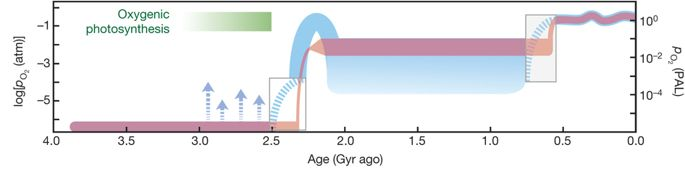
\includegraphics[width=0.8\textwidth]{nature13068-f1}
	\end{figure}
	
	\begin{figure}[H]
		\caption{Geologic aeons after \cite{nisbet2011evolution} showing emergence of metahogenesis}\label{fig:nisbet2011evolution}
		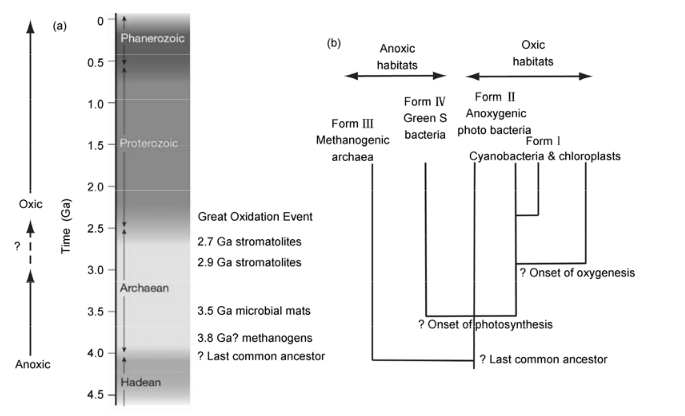
\includegraphics[width=0.8\textwidth]{nisbet2011evolution}
	\end{figure}
	
	\item Aerobic oxidation is unlikely to have arisen prior to oxygen becoming available. Moreover it requires two inventions, photo synthesis and oxidation itself, whereas methanogenesis requires only one, and is therefore simpler, all things being equal.
	
	\item A hint may be found in \cite{nisbet2011evolution}.\begin{quote}
		Sedimentological evidence implies there were liquid oceans despite the faint young Sun. These oceans may have been sustained by the greenhouse warming effect of biologically-made methane. Oxygenesis in the late Archaean would have released free O2 into the water. This would have created oxic surface waters, challenging the methane greenhouse. After the Great Oxidation Event around 2.3 to 2.4 billion years ago, the atmosphere itself became oxic, perhaps triggering a glacial crisis by cutting methane-caused greenhouse warming.
	\end{quote}
	Perhaps an "oxygen-first world" might have been too cold to progress.
	\item The following suggests that methanogenesis may in some sense be easy, as different organisms have different pathways.
	\begin{quote}
		Although the biochemical machinery in methanogens varies with the pathway used, few functional genes, which encode for key enzymes in the production of methane, are common to all known methanogens--\cite{angel2012methanogenic}
	\end{quote}
	On the other hand, a metabolism that consumes oxygen depends on mitochondria.
\end{enumerate}


\subsection{
	If aerobic oxidation is more energetically favorable, why would methanogenesis still exist today?
}
There are still plenty of anaerobic environments. It seems eminently reasonable that organisms could successfully practice oxygen-free lifestyles if there is no oxygen.
\begin{quote}
	Methanogens are strict anaerobes, and methanogenesis was shown to be fully suppressed upon exposure to oxygen in both pure culture and in soil--\cite{angel2012methanogenic}.
\end{quote}

\section{Life elsewhere}

You have been asked to participate on a mission to locate extraterrestrial life. What geochemical signatures would you want to look for to help you determine if a planet is or has been inhabited in the past, based on the fossil record of the Earth and geochemistries elsewhere in the solar system?

\begin{itemize}
	\item I'd want to look at stars that had enough time to evolve interesting life, so I'd avoid stars from spectral classes O, B, A, and maybe F0\cite{antf2019spectral}.  M-type stars have a very small habitable zone, exposing the planet to solar flares and other radiation. \cite{dvorskywim2015this}. K-type stars have a long life, and are more stable \cite{shiga2009orange} \cite{wiki:kTypeStar}. In short I'd want to focus on G (the only known living planet orbits a G2 star) and K.
	\item Many exoplants are not hospitable, such as hot Jupiters\cite{ wiki:hot:jupiter}, with a mass spanning $0.36\text{--}11.8M_{\jupiter}$ and periods of between 1.3 and 111 Earth days. I assume that we won't go to systems that consist entirely of hot Jupiters.
	\item If we have the luxury of being able to reach a solar system with a similar distribution to ours (terrestrial planets, then gas giants, then ice giants), I would vote for it, as the Nice model \cite{morbidelli2010coherent} and \cite{gomes2005origin} would suggest that the Late Heavy Bombardment was over.
	\item I'd prioritize terrestrial planets in the habitable zone--\cite{nasa2019goldilocks}, and which are large enough to possess an atmosphere, as these, by definition, are the planets that \textit{might} have liquid water.\footnote{This decision implicitly assumes that we are looking for \gls{gls:LAWKI}. } I would attach a lower priority to Mars-like planets that may have been in the habitable zone in the past, and I'd avoid Venus-like planets, which might once have been in the habitable zone but are now hot enough to kill me. I'd use a model of stellar evolution\cite{wiki:stellar:evolution} to determine when each planet was likely to have been habitable, and assume that it would be difficult to find fossils older than 1 billion years or so.
	\item I would perform a spectrographic analysis of the atmosphere of each planet. If I were lucky enough to find a blue planet with an atmosphere like ours I would head for it straight away\footnote{Unless there were alien megastructures--\cite{wiki:ringworld}: if so, be very, very careful!}, but I wouldn't count on it. Instead I would look at whether or not the atmosphere was in chemical equilibrium\cite{lovelock1974atmospheric}.
	\begin{itemize}
		\item If it is not in equilibrium, is there any obvious, non-biogenic explanation?
		\item If every planet in the habitable zone is in equilibrium we need a Plan B. If we have a mother ship and at least one lander, I'd be inclined to explore the Mars-like planet, while the mother ship monitors the other candidates. It is possible that there may be belches of gas similar to those observed on Mars--\cite{nasa2019curiosity}. If a planet belches a gas, an no convincing non-biogenic explanation found, it should be elevated. 
	\end{itemize}
	\item I'd want to rule out obvious killers: if the planet lacks a magnetic field, there may be excessive radiation bombardment; a planet that keeps one face turned towards its Sun, or is in an excessively eccentric orbit might not be a good bet, at least for \gls{gls:LAWKI}.  
\end{itemize}

\section{Phylogenic tree building}

\subsection{Phylogenic tree based on a single sequence}

Figure \ref{fig:Phylo1} was generated by \gls{gls:BLAST}, using 50S ribosomal protein L5 and the organisms listed in Table \ref{tab:organisms}. I chose the protein more or less arbitrarily, and then found organisms that were in the NCBI database and expressed the selected protein. I wanted representatives of all 3 super-kingdoms, archaea, bacteria, and eukaryotes.

\begin{table}[H]
	\caption{Organisms, using 50S ribosomal protein L5.}\label{tab:organisms}
	\centering
	\begin{tabular}{|l |r | p{5cm} |}
		\hline
		\textbf{Organism} & \textbf{GI} & \textbf{Remarks}\\ \hline
		Arabidopsis lyrata subsp. lyrata &297318733 & Eukaryote,  kingdom Plantae \\ \hline
		Arc I group archaeon ADurb1013\_Bin02101&1004829435&Archaeon\\ \hline
		Wolbachia endosymbiont of Drosophila melanogaster  &42410257 &Bacterium \\ \hline
		Drosophila silvestris&217426024&Eukaryote, kingdom Animalia\\\hline
		Escherichia coli &553605257 & Bacterium\\ \hline
		Pseudomonas aeruginosa &354823940 & Bacterium\\ \hline
		Shigella sonnei &903021862 &Bacterium \\ \hline
		Pyrococcus furiosus &499322460 &Archaeon \\ \hline
		Homo sapiens & 119593493&Eukaryote, kingdom Animalia  \\ \hline
		Entamoeba histolytica  &449706951&Eukaryote, phylum Amoebozoa\\ \hline
		Aigarchaeota archaeon NZ13\_MG1&1378806004&Archaeon\\ \hline
	\end{tabular}
\end{table}

\begin{figure}[H]
	\caption{Phylogenic tree based on 50S ribosomal protein L5.  Note that only one eukaryote appears, \textit{Arabidopsis lyrata}.}\label{fig:Phylo1}
	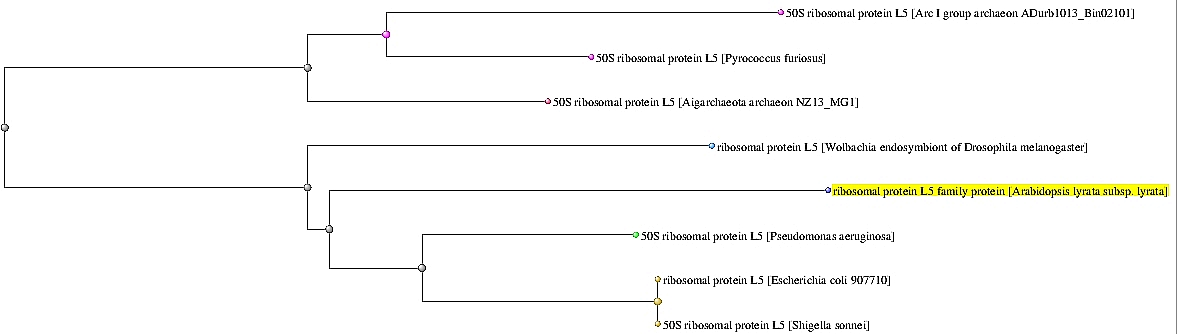
\includegraphics[width=\textwidth]{Phylo1}
\end{figure}

Note that BLAST has dropped all Eukaryotes  from the tree, except for  \textit{Arabidopsis lyrata}. I discuss this in Section \ref{sect:compare}.

\subsection{Generate a phylogenic tree based on the known taxonomy}

Figure \ref{fig:Phylo2} was generated using \cite{biobyte2019phylot}. Since the website restricted me to 9 species or fewer, I dropped two eukaryotes that were present in Table \ref{tab:organisms} but absent from Figure \ref{fig:Phylo1}.

\begin{figure}[H]
	\caption{Phylogenic tree based on the known taxonomy}\label{fig:Phylo2}
	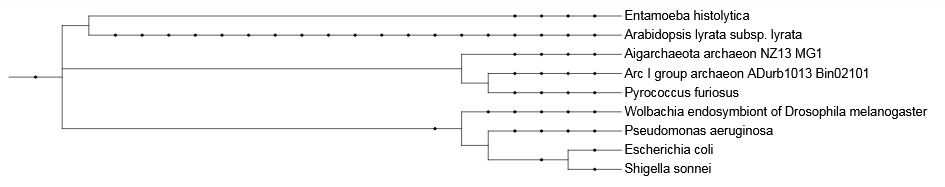
\includegraphics[width=\textwidth]{Phylo2}
\end{figure}

\subsection{Compare protein and taxonomic trees}\label{sect:compare}

\begin{enumerate}
	\item The most obvious difference between Figures \ref{fig:Phylo1} and  \ref{fig:Phylo2} is the number of nodes: neither \textit{Homo sapiens} nor \textit{Entamoeba histolytica} appear in Figure \ref{fig:Phylo1}. Since these are Eukaryotes, I assume that they were too distant from the other sequences, so BLAST dropped them from the tree. If this is the case, why is the eukaryote \textit{Arabidopsis lyrata} in the tree?
	\item Bacteria and archaea are generally organized similarly in  Figures \ref{fig:Phylo1} and  \ref{fig:Phylo2}.
	\item I conjecture that \textit{Arabidopsis lyrata} is present because it was entered as the Query Sequence--Figure \ref{fig:BLAST1}--and the other species were entered as Subject Sequences: the others were therefore judges against \textit{Arabidopsis lyrata}. The \textit{results} view reported 7 Sequences producing significant alignment, consistent with the 8 shown in Figure \ref{fig:Phylo1}.
	\item As an experiment I reran BLAST, but used \textit{Entamoeba histolytica } as the Query Sequence, and placed \textit{Arabidopsis lyrata} among the Subject Sequences. Figure \ref{fig:Phylo3} shows the results: three eukaryotes-- Homo, our "cousins" Drosophila, and Entamoeba--together with one Bacterium, \textit{Pseudomonas aeruginosa}. 
	\item Since Figures \ref{fig:Phylo1} and \ref{fig:Phylo3} suggest that \textit{Pseudomonas aeruginosa} is a rather sociable chap, I tried putting him in the Query Sequence, as shown im Figure \ref{fig:Phylo4}. The archaea are grouped together, as are most eukaryotes, except for \textit{Drosophila silvestris}, which is anomalous. Bacteria are oddly split between ones that are close to archaea, and others that are more remote.
\end{enumerate}

\begin{figure}[H]
	\caption{BLAST Query}\label{fig:BLAST1}
	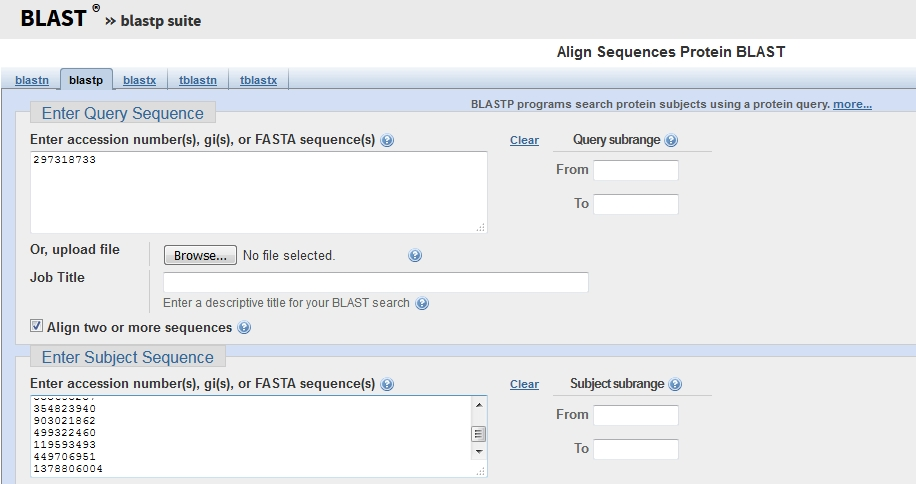
\includegraphics[width=0.8\textwidth]{BLAST1}
\end{figure}

\begin{figure}[H]
	\caption{Phylogenic tree using \textit{Entamoeba histolytica}}
	\label{fig:Phylo3}
	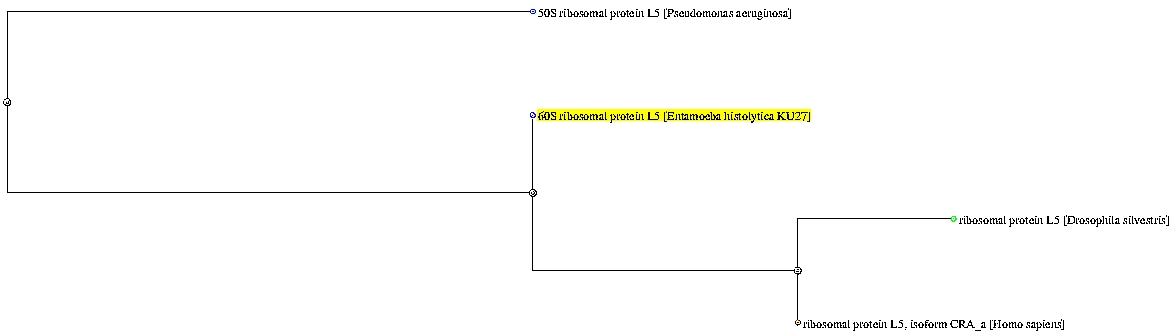
\includegraphics[width=\textwidth]{Phylo3}
\end{figure}

\begin{figure}[H]
	\caption{Phylogenic tree using \textit{Pseudomonas aeruginosa}}
	\label{fig:Phylo4}
	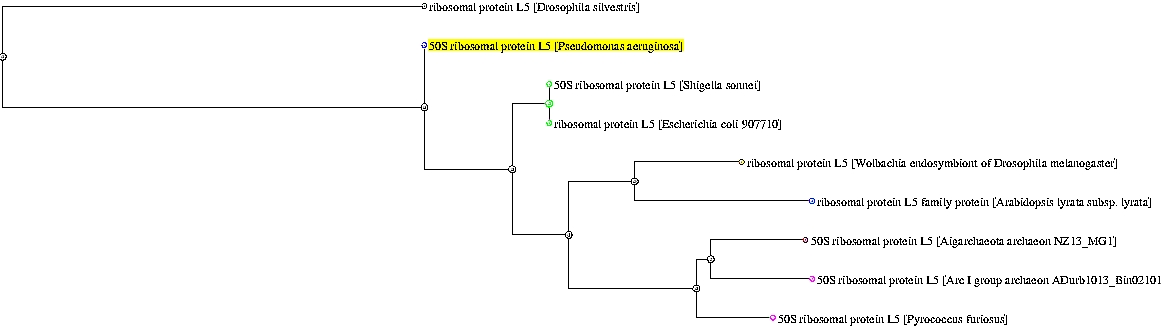
\includegraphics[width=\textwidth]{Phylo4}
\end{figure}

\subsection{Challenges building Phylogenic trees}

Section \ref{sect:compare} illustrates this. In comparing the 3 super-kingdomes we are dealing with very long branches, so drift and long branch attraction have time to confound individual sequences. Our hope is that we can harmonize partial trees based on many sequences.

% end of text 

% glossary
\printglossaries

% bibliography go here

\bibliographystyle{unsrt}
\addcontentsline{toc}{section}{Bibliography}
\bibliography{origins,wikipedia}

\end{document}
